\documentclass[12pt]{article}
\usepackage{amsfonts, epsfig}

\usepackage{graphicx}
\usepackage{fancyhdr}
\pagestyle{fancy}
\lfoot{\texttt{coms30127.github.io}}
\lhead{Computation Neuroscience - 04.1\_rate\_neurons - Conor}
\rhead{\thepage}
\cfoot{}

\usepackage{graphicx}

\usepackage{listings}

\usepackage{tikz}

\usepackage{pgf}
\usepackage[utf8]{inputenc}
\usetikzlibrary{arrows,automata}
\usetikzlibrary{positioning}


\tikzset{
    state/.style={
           rectangle,
           rounded corners,
           draw=black, very thick,
           inner sep=2pt,
           text centered,
           },
}
\tikzset{
    on/.style={
           circle,
           draw=red, very thick,
           inner sep=2pt,
           fill=red!25,
           },
}


\tikzset{
    off/.style={
           circle,
           draw=blue, very thick,
           inner sep=2pt,
           text centered,
           },
}



\tikzset{
    neuron/.style={
           rectangle,
           rounded corners,
           draw=black, very thick,
           inner sep=2pt,
           text centered,
           },
}



\tikzset{
    area/.style={
           rectangle,
           draw=black, very thick,
           inner sep=2pt,
           text centered,
           },
}


\tikzset{
    gc/.style={
           rectangle,
           rounded corners,
           draw=red, very thick,
           inner sep=2pt,
           text centered,
           },
}


\tikzset{
    inh/.style={
           rectangle,
           rounded corners,
           draw=blue, very thick,
           inner sep=2pt,
           text centered,
           },
}



\tikzset{
    io/.style={
           rectangle,
           draw=green, very thick,
           inner sep=2pt,
           text centered,
           },
}


\usepackage{ifthen}
\newboolean{nopics}
\setboolean{nopics}{false}



\begin{document}

\section*{Rate neurons} 

In this short note we introduce the idea of rate-based neurons. In the
previous section we considered McCulloch-Pitts neurons, these have an
on-off behaviour, we know that neurons actually communicate using
spikes, also called action potentials, discrete pulses of voltage. Of
course, this is not necessarily inconsistient; it is possible, but
unlikely, that neurons have a low and high firing rate and that we can
effectively analyse that part of the behaviour of the brain that is
relevant to computation by considering neurons only as on / off
thresholding units. Howver, it is much more likely that this would only give a
very partial account of neural computation, but that there are
nonetheless useful insights to be gained in considering what
algorithms could be supported by on-off neurons.

The next step in our consideration of neuronal models is to imagine
that spikes are irrelevant but spike firing rates are important and
that we can understand neural computation by describing computation
based on neural firing rates. It is known that this picture does not
apply to some specialised circuits such at the one used by owls to
locate their prey. In the owl auditory system the precise temporal
difference between sounds arriving at each of the owls ears is
calculated by finding the point individual spikes from each ear arrive
at the same point. However, it is not uncommon for people to believe
that, in general, neuronal computation is based on the communication
and transformation of firing rates; in fact, one very common
point-of-view is that computation is rate based but that plasticity,
that is learning through changes in synapse strengths, depends on spike times.

The idea of rate coding dates back to the earliest detailed
measurements of the electrical activity of nervous system. Edgar
Adrian was one of the great pioneers, he was a neurophysiologist, but,
as is often the case, his success relied on innovation in equipment,
coupled, of course, to careful experimentation. He pioneered the use
of vaccuum tubes to amplify electical signals allowing him and his
co-workers to record the activity in individual nerve fibres. He
recorded from the sensory nerves carrying signals from muscles in
frog, by attaching a silk thread to the muscle, passing it over a
pulley and attaching a weight he was able to observe a linear
relationship between the frequency of spikes along the nerve and the
size of the weight. He also noted that the frequency decreased with
time, see Fig.~\ref{fig_adrian}.

\begin{figure}[tb]
\ifthenelse{\boolean{nopics}}
             {\textsl{This graph has two curves, one labelled 3 grams, the other 0.5 grams. The y-axis is titled ``frequency per second'' and has marks spanning zero to 150, the x-axis is titled seconds after loading and runs for 20 seconds. It is indicated that the load is removed at 20 seconds. Both curves are smooth and decay gently, they are both surrounded by dots giving the acual data. The 3 gram curve is higher than the 0.5 gram, it starts near 150 and decays to about 90; the 0.5 gram starts at 70 and decays to about 30.}}
             {
               \begin{center}
                 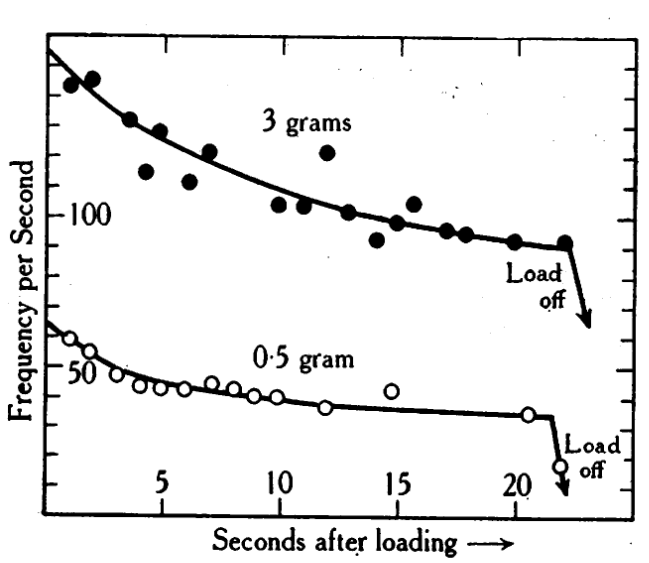
\includegraphics[width=8cm]{Adrian.png}
               \end{center}
             }
             \caption{A figure from \cite{AdrianZotterma1926} showing
               the response to two different weights.\label{fig_adrian}}
\end{figure}
\begin{thebibliography}{10}

\bibitem{AdrianZotterma1926}
  Adrian, ED. and Zotterman Y (1926) The impulses produced by sensory nerve-endings: Part II. The response of a Single End-Organ.
\newblock The Journal of Physiology, 61.2:151


\end{thebibliography}


\end{document}
